%!TEX root = ../main.tex
% Chapter 1

%\chapter{background}
\chapter{Introduction}







\chapter{Literature Study}
\section{Modeling the DC Motor}
According to the Prescribed textbook\cite[p.160]{dorf2011modern}, \quote{\emph{Time constant} The time interval necessary for a system to
change from one state to another by a specified percentage. For a first order system, the time constant is
the time it takes the output to manifest a 63.2\%
change due to a step input.}




\chapter{Modeling}
In this section the characteristics of the DC motor need to be interpreted in a way that allows an appropriate controller to built around it. The List of all the measured parameters, and methods are included in the ``One page Experiment design'' included in \hyperref[apx:A]{Appendix A}.Since the specification only requires a first order model of the motor, and since the mechanical time constant overwhelms the electrical time constant, the mechanical time constant is the only parameter necessary to meet the specifications.
\section{Measuring the Mechanical Time constant}
With regards to the definition of a time constant as discussed in the Literature study, the time constant of the DC motor was calculated by plotting the rotational velocity of the over time after shutting off the power source. Refer to Figure~\ref{fig:shutoff}
These Measurements were taken by connecting the Tachometer to the PicoScope and recording the values into a .csv file. The Data was prepared for plotting in the following ways:
\begin{itemize}
	\item The time stamps were offset so that the shutoff occurred at $t=0$ 
	\item The tachometer gave a reading 360mV when the speed was 0 RPM, so the Y axis was offset accordingly
	\item The Data was smoothed using an average filter. See python script in \hyperref[apx:B]{Appendix B}
\end{itemize}

\begin{figure}[h]
    \myfloatalign
    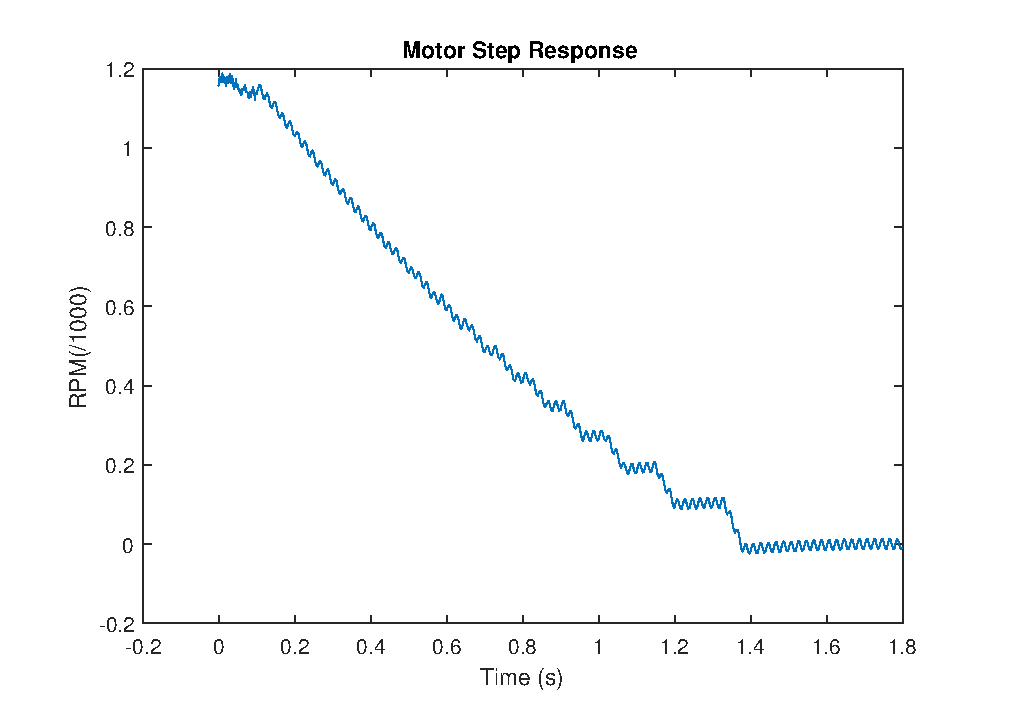
\includegraphics[width=1.2\textwidth]{gfx/Motor_shutoff} %can also be placed in images/example
    \caption{Time Response of the DC motor}
    \label{fig:shutoff}
\end{figure}
From the representation of the data in Figure~\ref{fig:shutoff}, it can be measured that the motor took Approximately 0.77 seconds to reach a speed of 440RPM, A value 63\% from the steady state value. The mechanical time constant $\tau_\ell$ is given by:
\begin{equation}
	\tau_\ell = 0.77s
\end{equation}
\section{Determining K and comparing the model with the results}
Having measured the time constant, the time domain model of the DC motor is in the form:
\begin{align}
	\dot{\omega}(t) &= Ke^{\frac{t}{\tau_\ell} }
\end{align}
Using the value calculated for $\tau_\ell$ and choosing K by means of trial and error, the following model was found to be reasonably close to the measured response:
\begin{align}\label{eq:1}
	K &= 1.2\\
	\dot{\omega}(t) &= 1.2e^{\frac{t}{0.77} }\\
	G(s) &= \frac{1.2}{0.77s+1} 
\end{align}
Refer to Figure~\ref{fig:shutoff_vs_model}, where the time domain model is compared to the measured results. 


\begin{figure}[h]
    \myfloatalign
    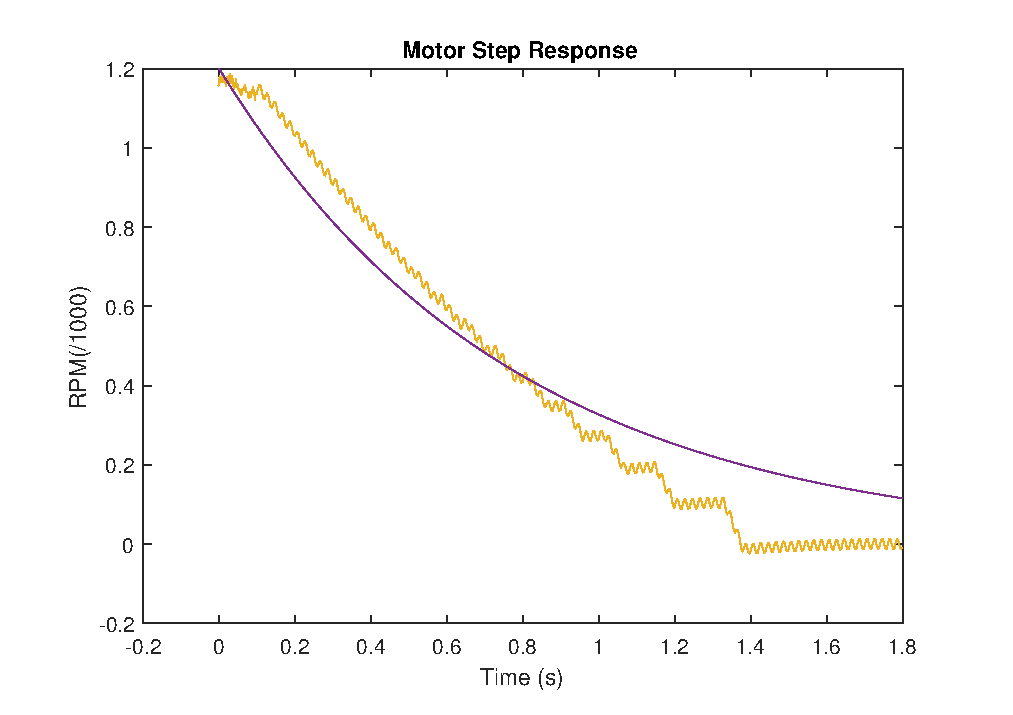
\includegraphics[width=1.2\textwidth]{gfx/Motor_shutoff_vs_Time_domain_model} %can also be placed in images/example
    \caption{Comparison of time domain model with Laboratory results}
    \label{fig:shutoff_vs_model}
\end{figure}
\section{Designing the PID}
The following table shows the specifications that the system must adhere to:

\begin{table}[h]
\centering
\caption{Specifications}
\label{tbl:1}
\begin{tabular}{llll}
\cline{1-2}
\multicolumn{1}{|l|}{\textbf{Parameter}}      & \multicolumn{1}{l|}{\textbf{Maximum Value}} &  &  \\ \cline{1-2}
\multicolumn{1}{|l|}{Steady state error}    & \multicolumn{1}{l|}{1\%}                   &  &  \\ \cline{1-2}
\multicolumn{1}{|l|}{Percent Overshoot(P.O.)} & \multicolumn{1}{l|}{10 \%}                       &  &  \\ \cline{1-2}
\multicolumn{1}{|l|}{Settling time} & \multicolumn{1}{l|}{<2s}                       &  &  \\ \cline{1-2}
                                              &                                             &  & 
\end{tabular}
\end{table}
The transfer function for a PI controller in General is given by:
\begin{equation}\label{eq:2}
	G_{c}(s) = K_{c}+ \frac{K_{i}}{s}
\end{equation}
The equations for Percent overshoot and settling time are given by:
\begin{align} \label{eq:3}
P.O. &= e^{\left( \frac{-\pi\zeta}{\sqrt{1-\zeta^2}}\right)}
\end{align}
\begin{align}\label{eq:6}
T_s &= \frac{4}{\zeta\omega_n}
\end{align}

Furthermore, $\zeta$ and $\omega_n$ can be used to define a desired characteristic equation in the form:

\begin{align} \label{eq:4}
Q(s) &= s^2 + 2\zeta\omega_ns + \omega_n^2
\end{align}

The PI controller design can be summed up as the reconciliation of the desired characteristic equation \ref{eq:4} with the characteristic equation of the system, which is given by:
\begin{align}\label{eq:5}
Q(s) &= G(s)G_c(s) + 1 
\end{align}
With respect to the equations \ref{eq:1} and \ref{eq:2}


%----------------------------------------------------------------------------------------

\chapter{Controller Design}
\chapter{Controller Simulation}
\chapter{Results}
\chapter{Discussion of results}
%\chapter{Literature review}
\chapter{Conclusion}


